\documentclass[12pt]{article}

\usepackage[utf8]{inputenc}
\usepackage[english,russian]{babel}
\usepackage{amsmath}
\usepackage[unicode, pdftex]{hyperref}
\usepackage[usenames]{color}
\usepackage{colortbl}
\usepackage{amssymb}
\usepackage[left=2.5cm, top=2cm, right=1cm, bottom=20mm, nohead, nofoot]{geometry}
\usepackage{svg}
\usepackage{graphicx}%Вставка картинок правильная
\usepackage{xcolor} % поддержка цвета
\graphicspath{{figs/}} % путь, где искать картинки
\usepackage{listings}

\begin{document}

\section{Нестационарное уравнение диффузии-конвекции-реакции для трехмерной расчетной области}

\subsection{Постановка задачи}

Уравнение диффузии-конвекции-реакции:


\begin{equation}
	c_t' + uc_x' + vc_y' + wc_z' = (\mu c_x')_x' + (\mu c_y')_y' + (\nu c_z')_z' + f,	
\end{equation}
с граничными условиями:

\begin{equation}
	c_n'(x, y, z, t) = \alpha_n c + \beta_n,
\end{equation}
где
\textit{u, v, w} - проекция вектора скорости на оси координат x, y и z соответственно,
\textit{f} - функция, описывающая интенсивность и распределение источников,
${\mu}$ - горизонтальная проекция коэффициента диффузионного (турбулентного) обмена,
${\nu}$ - вертикальная проекция коэффициента диффузионного (турбулентного) обмена.

\subsection{Построение дискретной модели}

Расчетная область вписана в прямоугольный параллелепипед. Для программной реализации математической модели транспорта веществ вводим равномерную расчетную сетку:

\begin{displaymath}
	\begin{split}
	w_h = \{t^n = n \tau, x_i = ih_x, y_j = jh_y, z_k = kh_z, n = \overline{0..N_t-1}, i = \overline{0..N_x-1},  \nonumber\\
	j = \overline{0..N_y-1}, k = \overline{0..N_z-1}, (N_t-1) \tau = l_x, (N_y-1)h_y = l_y, (N_z-1)h_z = l_z \}, \nonumber\\
	\end{split}
\end{displaymath}
где
${\tau}$ - шаг по временному направлению;
${h_x, h_y, h_z}$ - шаги по координатным осям пространства;
${N_t, N_x, N_y, N_z}$ - чмсло узлов расчетной сетки  по времени $t$ и пространственным координатам $x$, $y$ и $x$ соответственно.

Аппроксимация уравнения (1) по временной переменной выполняется на основе схем с весами. 

\begin{equation}
	\frac{\hat c - c}{\tau} + u\bar{c}_x' + v\bar{c}_y' + w\bar{c}_z' = (\mu\bar{c}_x')_x' + (\mu\bar{c}_y')_y' + (\nu\bar{c}_z')_z' + f ,		
\end{equation}
где  

$\bar{c} = \sigma\hat c + (1 - \sigma)\cdot c , \sigma \in [0,1] $ - вес схемы $(\sigma = 0,5; 0.75; 1)$

$c=c(x, y, z, t);$ $ $ $\hat c = (x, y, z, t + \tau)  $


\begin{figure}[h!]
	\centering
	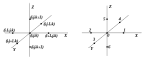
\includegraphics {figs/shablon}
	\caption{ Разностный шаблон}
\end{figure}

<<<<<<< HEAD
=======
\begin{figure}[h!]
	\centering
	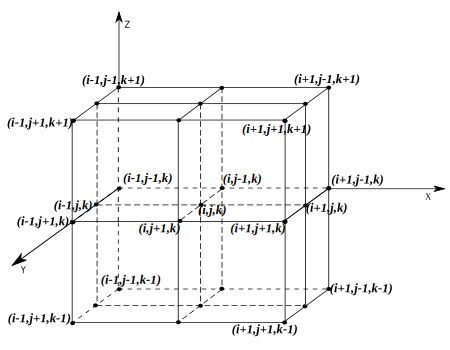
\includegraphics {figs/ris2}
	\caption{ Параллилепипед с центром i, j, k}
\end{figure}
>>>>>>> 7f08de0ad0f7ca17b5bd5dccabc93e1c3458492e

Ячейки представлены прямоугольными параллелепипедами, которые могут быть заполненными, пустыми или частично заполненными (см. рисунок 1). 

\begin{figure}[h!]
	\centering
	\includegraphics {figs/ris3}
	\caption{ Вершины объемной ячейки}
\end{figure} 

\begin{figure}[h!]
	\centering
	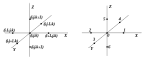
\includegraphics {figs/shablon}
	\caption{ Разностный шаблон}
\end{figure}

\begin{figure}[h!]
	\centering
	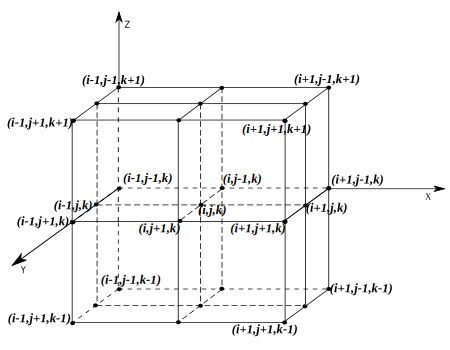
\includegraphics {figs/ris2}
	\caption{ Параллилепипед с центром i, j, k}
\end{figure}

Заполненность ячеек:
Центры ячеек и расчетные узлы сетки разнесены на $ \frac{h_x}{2}, \frac{h_y}{2}, \frac{h_z}{2} $ по координатным направлениям $x, y, z$ соответственно.

Обозначим $O_{i,j,k}$ - степень заполненности объемной ячейки. 

<<<<<<< HEAD
=======
\begin{figure}[h!]
	\centering
	\includegraphics {figs/ris3}
	\caption{ Вершины объемной ячейки}
\end{figure}

>>>>>>> 7f08de0ad0f7ca17b5bd5dccabc93e1c3458492e

Получается, что окрестными ячейками узла ${i,j,k}$ являются 8 ячеек (см. рисунок 2).

Обозначим эти ячейки через координаты главных диагоналей (т. к. ячейки - это прямоугольные параллелепипеды).
\\*
\newpage
Внизу:

1) ${(i-1,j+1,k-1)}$ - ${(i,j,k)}$ 

2) ${(i-1,j,k-1)}$ - ${(i,j-1,k)}$ 

3) ${(i,j,k-1)}$ - ${(i+1,j-1,k)}$ 

4) ${(i,j+1,k-1)}$ - ${(i+1,j,k)}$ 

Вверху:

1) ${(i-1,j+1,k)}$ - ${(i,j,k+1)}$ 

2) ${(i-1,j,k)}$ - ${(i,j-1,k+1)}$ 

3) ${(i,j,k)}$ - ${(i+1,j-1,k+1)}$ 

4) ${(i,j+1,k)}$ - ${(i+1,j,k+1)}$ 

{\color{red}{Читай метод конечных объемов (Рояк)}}


Для описания геометрии расчетного объема введем коэффициенты ${q_0, q_1,q_2,q_3,q_4,q_5,q_6}$ заполненности контрольных  ''объемов'' ячейки ${(i,j,k)}$.

Значение ${q_i}$ характеризует степень заполненности объема ${V_i}$, где $i=\overline{0...6}$.

\begin{equation*}
{q_0} - {V_0}: x\in (x_{i-\frac{1}{2} }, x_{i+\frac{1}{2} } ),  y\in (y_{j-\frac{1}{2} }, y_{j+\frac{1}{2} } ),  z\in (z_{k-\frac{1}{2} }, z_{k+\frac{1}{2} } )
\end{equation*}

\begin{equation*}
{q_6} - {V_1}: x\in (x_{i-\frac{1}{2} }, x_{i+\frac{1}{2} } ),  y\in (y_{j-\frac{1}{2} }, y_{j+\frac{1}{2} } ),  z\in (z_{k-\frac{1}{2} }, z_k )
\end{equation*}

\begin{equation*}
{q_5} - {V_2}: x\in (x_{i-\frac{1}{2} }, x_{i+\frac{1}{2} } ),  y\in (y_{j-\frac{1}{2} }, y_{j+\frac{1}{2} } ),  z\in (z_k, z_{k+\frac{1}{2} } )
\end{equation*}

\begin{equation*}
{q_2} - {V_3}: x\in (x_{i-\frac{1}{2} }, x_i ),  y\in (y_{j-\frac{1}{2} }, y_{j+\frac{1}{2} } ),  z\in (z_{k-\frac{1}{2} }, z_{k+\frac{1}{2} } )
\end{equation*}

\begin{equation*}
{q_1} - {V_4}: x\in (x_i, x_{i+\frac{1}{2} } ),  y\in (y_{j-\frac{1}{2} }, y_{j+\frac{1}{2} } ),  z\in (z_{k-\frac{1}{2} }, z_{k+\frac{1}{2} } )
\end{equation*}

\begin{equation*}
{q_4} - {V_5}: x\in (x_{i-\frac{1}{2} }, x_{i+\frac{1}{2} } ),  y\in (y_{j-\frac{1}{2} }, y_j ),  z\in (z_{k-\frac{1}{2} }, z_{k+\frac{1}{2} } )
\end{equation*}

\begin{equation*}
{q_3} - {V_6}: x\in (x_{i-\frac{1}{2} }, x_{i+\frac{1}{2} } ),  y\in (y_j, y_{j+\frac{1}{2} } ),  z\in (z_{k-\frac{1}{2} }, z_{k+\frac{1}{2} } )
\end{equation*}

Будем называть $\Omega$ заполненные части объемов $V_m$, где $m=\overline{0...6}$. 
Таким образом, коэффициенты $g_m$ вычисляются по формулам:

\begin{equation*}
(q_0)_{i,j,k}=\frac{O_{i,j,k}+O_{i+1,j,k}+O_{i,j+1,k}+O_{i+1,j+1,k}+O_{i,j,k+1}+O_{i+1,j,k+1}+O_{i,j+1,k+1}+O_{i+1,j+1,k+1}}{8};
\end{equation*}

\begin{equation*}
 (q_6)_{i,j,k}=\frac{O_{i,j,k+1}+O_{i+1,j,k+1}+O_{i,j+1,k+1}+O_{i+1,j+1,k+1}}{4};
\end{equation*}

\begin{equation*}
(q_5)_{i,j,k}=\frac{O_{i,j,k}+O_{i+1,j,k}+O_{i,j+1,k}+O_{i+1,j+1,k}}{4};
\end{equation*}

\begin{equation*}
(q_2)_{i,j,k}=\frac{O_{i,j,k+1}+O_{i,j+1,k}+O_{i,j,k+1}+O_{i,j+1,k+1}}{4};
\end{equation*}

\begin{equation*}
(q_1)_{i,j,k}=\frac{O_{i+1,j,k}+O_{i+1,j+1,k}+O_{i+1,j,k+1}+O_{i+1,j+1,k+1}}{4};
\end{equation*}

\begin{equation*}
(q_4)_{i,j,k}=\frac{O_{i,j,k}+O_{i+1,j,k}+O_{i,j,k+1}+O_{i+1,j,k+1}}{4};
\end{equation*}

\begin{equation*}
(q_3)_{i,j,k}=\frac{O_{i,j+1,k}+O_{i+1,j+1,k}+O_{i,j+1,k+1}+O_{i+1,j+1,k+1}}{4};
\end{equation*}

Проинтегрируем по объему $\Omega_0$ уравнение (2), воспользуемся свойством линейности интеграла, в результате чего получим:

\begin{multline}
\iiint\limits_{\Omega_0} \frac{\hat c - c}{\tau}\,dxdydz + \iiint\limits_{\Omega_0} u\bar{c}_x'\,dxdydz + \iiint\limits_{\Omega_0} v\bar{c}_y'\,dxdydz + \iiint\limits_{\Omega_0} w\bar{c}_z'\,dxdydz = \\
\iiint\limits_{\Omega_0} (\mu\bar{c}_x')_x'\,dxdydz + \iiint\limits_{\Omega_0} (\mu\bar{c}_y')_y'\,dxdydz + \iiint\limits_{\Omega_0} (\mu\bar{c}_z')_z'\,dxdydz + \iiint\limits_{\Omega_0} f\,dxdydz  
\end{multline}

Вычислим отдельно каждый из полученных интегралов.

\begin{equation}
	\iiint\limits_{\Omega_0} \frac{\hat c - c}{\tau}\,dxdydz \simeq (q_0)_{i,j,k}\iiint\limits_{V_0} \frac{\hat c - c}{\tau}\,dxdydz = (q_0)_{i,j,k}\frac{\hat c - c}{\tau}h_xh_yh_z
\end{equation}
Второй интеграл в формуле (4) принимает вид:

\begin{multline*}
\iiint\limits_{\Omega_0} u\bar{c}_x'\,dxdydz \simeq \iiint\limits_{\Omega_1} u\bar{c}_x'\,dxdydz + \iiint\limits_{\Omega_2} u\bar{c}_x'\,dxdydz \\  
= (q_1)_{i,j,k}\iiint\limits_{V_1} u\bar{c}_x'\,dxdydz + (q_2)_{i,j,k}\iiint\limits_{V_2} u\bar{c}_x'\,dxdydz
\end{multline*}

Вычислим интегралы по $V_1$ и $V_2$:

\begin{equation*}
	\iiint\limits_{V_2} u\bar{c}_x'\,dxdydz = \int\limits_{z_{k-\frac{1}{2}}}^{z_{k+\frac{1}{2}}}dz \int\limits_{y_{j-\frac{1}{2}}}^{y_{j+\frac{1}{2}}}dy   \int\limits_{x_{i-\frac{1}{2}}}^{x_{i}}u\bar{c}_x'dx \simeq u_{{i-\frac{1}{2}},j,k}\frac{\bar{c}_{i,j,k}-\bar{c}_{i-1,j,k}}{2}h_yh_z
\end{equation*}

\begin{equation*}
\iiint\limits_{V_1} u\bar{c}_x'\,dxdydz = \int\limits_{z_{k-\frac{1}{2}}}^{z_{k+\frac{1}{2}}}dz \int\limits_{y_{j-\frac{1}{2}}}^{y_{j+\frac{1}{2}}}dy   \int\limits_{x_i}^{x_{i+\frac{1}{2}}}u\bar{c}_x'dx \simeq u_{{i+\frac{1}{2}},j,k}\frac{\bar{c}_{i+1,j,k}-\bar{c}_{i,j,k}}{2}h_yh_z
\end{equation*}

Следовательно,

\begin{equation}
	\iiint\limits_{\Omega_0} u\bar{c}_x'\,dxdydz = (q_2)_{i,j,k}u_{{i-\frac{1}{2}},j,k}\frac{\bar{c}_{i,j,k}-\bar{c}_{i-1,j,k}}{2}h_yh_z +
	(q_1)_{i,j,k}u_{{i+\frac{1}{2}},j,k}\frac{\bar{c}_{i+1,j,k}-\bar{c}_{i,j,k}}{2}h_yh_z,
\end{equation}

где 
\begin{equation*} 
	u_{{i+\frac{1}{2}},j,k} = \frac{u_{i+1,j,k}+u_{i,j,k}}{2};
\end{equation*}

\begin{equation*} 
	u_{{i-\frac{1}{2}},j,k} = \frac{u_{i-1,j,k}+u_{i,j,k}}{2};
\end{equation*}


Аналогично вычислим

\begin{multline*}
	\iiint\limits_{\Omega_0} v\bar{c}_y'\,dxdydz = 
	\iiint\limits_{\Omega_3} v\bar{c}_y'\,dxdydz + 
	\iiint\limits_{\Omega_4} v\bar{c}_y'\,dxdydz \\  
	= (q_5)_{i,j,k}\iiint\limits_{V_3} v\bar{c}_y'\,dxdydz +
	 (q_4)_{i,j,k}\iiint\limits_{V_4} v\bar{c}_y'\,dxdydz = \\
	 (q_4)_{i,j,k}\int\limits_{z_{k-\frac{1}{2}}}^{z_{k+\frac{1}{2}}}dz\int\limits_{x_{i-\frac{1}{2}}}^{x_{i+\frac{1}{2}}}dx\int\limits_{y_{j-\frac{1}{2}}}^{y_j}v\bar{c}_y'dy + (q_3)_{i,j,k}\int\limits_{z_{k-\frac{1}{2}}}^{z_{k+\frac{1}{2}}}dz\int\limits_{x_{i-\frac{1}{2}}}^{x_{i+\frac{1}{2}}}dx\int\limits_{y_j}^{y+\frac{1}{2}}v\bar{c}_y'dy = \\
	 (q_4)_{i,j,k}v_{i,j-\frac{1}{2},k}\frac{\bar{c}_{i,j-1,k}+\bar{c}_{i,j,k}}{2}h_xh_z + (q_3)_{i,j,k}v_{i,j+\frac{1}{2},k}\frac{\bar{c}_{i,j+1,k}+\bar{c}_{i,j,k}}{2}h_xh_z,
\end{multline*}

где 
\begin{equation*} 
	v_{{i,j+\frac{1}{2}},k} = \frac{v_{i,j+1,k}+v_{i,j,k}}{2};
\end{equation*}

\begin{equation*} 
	v_{{i,j-\frac{1}{2}},k} = \frac{v_{i,j-1,k}+v_{i,j,k}}{2};
\end{equation*}

Аналогично вычислим:

\begin{multline*}
	\iiint\limits_{\Omega_0} w\bar{c}_x'\,dxdydz = \iiint\limits_{\Omega_5} w\bar{c}_x'\,dxdydz + \iiint\limits_{\Omega_6} w\bar{c}_x'\,dxdydz = \\
	(q_5)_{i,j,k}\iiint\limits_{V_5} w\bar{c}_z'\,dxdydz +
	(q_6)_{i,j,k}\iiint\limits_{V_6} w\bar{c}_z'\,dxdydz = \\
	(q_6)_{i,j,k}\int\limits_{y_{j-\frac{1}{2}}}^{y_{j+\frac{1}{2}}}dy\int\limits_{x_{i-\frac{1}{2}}}^{x_{i+\frac{1}{2}}}dx\int\limits_{z_{k-\frac{1}{2}}}^{z_k}w\bar{c}_z'dz + (q_5)_{i,j,k}\int\limits_{y_{j-\frac{1}{2}}}^{y_{j+\frac{1}{2}}}dy\int\limits_{x_{i-\frac{1}{2}}}^{x_{i+\frac{1}{2}}}dx\int\limits_{z_k}^{z_{k+\frac{1}{2}}}w\bar{c}_z'dz = \\
	(q_6)_{i,j,k}w_{i,j,k-\frac{1}{2}}\frac{\bar{c}_{i,j,k-\frac{1}{2}}+\bar{c}_{i,j,k}}{2}h_xh_y + (q_5)_{i,j,k}w_{i,j,k+\frac{1}{2}}\frac{\bar{c}_{i,j,k+\frac{1}{2}}+\bar{c}_{i,j,k}}{2}h_xh_y,
\end{multline*}

где 
\begin{equation*} 
	w_{{i,j},k+\frac{1}{2}} = \frac{w_{i,j,k+1}+w_{i,j,k}}{2};
\end{equation*}

\begin{equation*} 
	w_{{i,j},k-\frac{1}{2}} = \frac{w_{i,j,k-1}+w_{i,j,k}}{2};
\end{equation*}

Вычислим интеграл, стоящий в правой части формулы (1):

\begin{equation*} 
	\iiint\limits_{\Omega_0} (\mu\bar{c}_x')_x'\,dxdydz = \iiint\limits_{\Omega_1} (\mu\bar{c}_x')_x'\,dxdydz + \iiint\limits_{\Omega_2} (\mu\bar{c}_x')_x'\,dxdydz
\end{equation*}

Рассмотрим случай: $V_{\Omega1}>V_{\Omega2}$, выделим из  $\Omega_1$ фрагмент $\Omega_{1,2}$ смежный  с областью $\Omega_2$,  при этом   $V_{\Omega2}=V_{\Omega{1,2}}$

\begin{multline*} 
	\iiint\limits_{\Omega_0} (\mu\bar{c}_x')_x'\,dxdydz = \iiint\limits_{\Omega_1\setminus\Omega_{1,2}} (\mu\bar{c}_x')_x'\,dxdydz + \iiint\limits_{\Omega_{1,2}\cup\Omega_2}(\mu\bar{c}_x')_x'\,dxdydz = \\
	((q_1)_{i,j,k} - (q_2)_{i,j,k})\iiint\limits_{V_1} (\mu\bar{c}_x')_x'\,dxdydz + (q_2)_{i,j,k}\iiint\limits_{V_0} (\mu\bar{c}_x')_x'\,dxdydz
\end{multline*}

Вычислим инртеграл:
\begin{equation*}
\iiint\limits_{V_0} (\mu\bar{c}_x')_x'\,dxdydz = \int\limits_{z_{k-\frac{1}{2}}}^{z_{k+\frac{1}{2}}}dz \int\limits_{y_{j-\frac{1}{2}}}^{y_{j+\frac{1}{2}}}dy\int\limits_{x_{i-\frac{1}{2}}}^{x_{i+\frac{1}{2}}}(\mu\bar{c}_x')_x'dx = \int\limits_{z_{k-\frac{1}{2}}}^{z_{k+\frac{1}{2}}}dz \int\limits_{y_{j-\frac{1}{2}}}^{y_{j+\frac{1}{2}}}(\mu\bar{c}_x')\bigg|_{x_{i-\frac{1}{2}}}^{x_{i+\frac{1}{2}}}dy
\end{equation*}

Введем замену:
$W=\mu\bar{c}_x'$

\begin{equation*}
	\int\limits_{z_{k-\frac{1}{2}}}^{z_{k+\frac{1}{2}}}dz \int\limits_{y_{j-\frac{1}{2}}}^{y_{j+\frac{1}{2}}}W\bigg|_{x_{i-\frac{1}{2}}}^{x_{i+\frac{1}{2}}}dy = \int\limits_{z_{k-\frac{1}{2}}}^{z_{k+\frac{1}{2}}}dz \int\limits_{y_{j-\frac{1}{2}}}^{y_{j+\frac{1}{2}}}(W_{i+\frac{1}{2}}- W_{i-\frac{1}{2}})dy = (W_{i+\frac{1}{2}}- W_{i-\frac{1}{2}})h_yh_z
\end{equation*}	
	
	Вычислим $W_{i+\frac{1}{2}}$ на отрезке $[x_{i+1},x_i]$:
	
\begin{equation*}
	\int_{x_i}^{x_{i+1}}\frac{W}{\mu}dx = \int_{x_i}^{x_{i+1}}\bar{c}_x'dx
\end{equation*}

или

\begin{equation*}
	\int_{x_i}^{x_{i+1}}W\frac{1}{\mu}dx = \int_{x_i}^{x_{i+1}}\bar{c}_x'dx,
\end{equation*}
следовательно, по теореме о среднем

\begin{equation*}
	W_{i+\frac{1}{2}}\int_{x_i}^{x_{i+1}}\frac{dx}{\mu}=\int_{x_i}^{x_{i+1}}\bar{c}_x'dx,
\end{equation*}
следовательно, $W_{i+\frac{1}{2}}$ вычисляется в точке $x_{i+\frac{1}{2}}$, так как считаем, что функция $W(x)$ - линейная. 
В противном случае, это будет не середина отрезка  $[x_{i+1},x_i]$.
 
Поделим обе части равенства на $\int_{x_i}^{x_{i+1}}\frac{dx}{\mu}$ и получим:

\begin{equation*}
	W_{i+\frac{1}{2}}=\left(\int_{x_i}^{x_{i+1}}\frac{dx}{\mu}\right)^{-1}\cdot\int_{x_i}^{x_{i+1}}\bar{c}_x'dx,
\end{equation*}

проинтегрируем $\bar{c}_x'$ и получим 

\begin{equation*}
	W_{i+\frac{1}{2}}=\frac{\bar{c}_{i+1} - \bar{c}_{i}}{\int_{x_i}^{x_{i+1}}\frac{dx}{\mu}}=\frac{\bar{c}_{i+1} - \bar{c}_{i}}{\frac{1}{\mu_{i+\frac{1}{2}}}\int_{x_i}^{x_{i+1}}dx} = \frac{\bar{c}_{i+1}-\bar{c}_{i}} {\frac{1}{\mu_{i+\frac{1}{2}}}x\bigg|_{x_{i}}^{x_{i+1}}} = \frac{\bar{c}_{i+1} - \bar{c}_{i}} {\frac{1}{\mu_{i+\frac{1}{2}}} (x_{i+1} - x_i)} =\mu_{i+\frac{1}{2}} \frac{\bar{c}_{i+1} - \bar{c}_{i}} {h_{x}},
\end{equation*}
где $h_{x}=x_{i+1}- x_i$.

Теперь вычислим $W_{i-\frac{1}{2}}$  на отрезке $[x_{i-1}, x_i]$.

\begin{equation*}
\int_{x_{i-1}}^{x_{i}}\frac{W}{\mu}dx = \int_{x_{i-1}}^{x_{i}}\bar{c}_x'dx
\end{equation*}

Вычисления для $W_{i-\frac{1}{2}}$ выполняем аналогично, как для $W_{i+\frac{1}{2}}$. Поэтому получим:

\begin{equation*}
	W_{i-\frac{1}{2}} = \mu_{i-\frac{1}{2}} \frac{\bar{c}_{i} -\bar{c}_{i-1} }{h_{x}}	
\end{equation*}

В результате получим:

\begin{multline*} 
	\iiint\limits_{V_0} (\mu\bar{c}_x')_x'\,dxdydz = (W_{i+\frac{1}{2}} - W_{i-\frac{1}{2}})h_yh_z=  \\   \left(\mu_{i+\frac{1}{2},j,k}\frac{(\bar{c}_{i+1,j,k}- \bar{c}_{i,j,k})}{h_x} - \mu_{i-\frac{1}{2},j,k}\frac{(\bar{c}_{i,j,k}- \bar{c}_{i-1,j,k})}{h_x}\right)h_yh_z
\end{multline*} 

Вычислим интеграл по $V_1$:

\begin{multline*} 
	\iiint\limits_{V_1} (\mu\bar{c}_x')_x'\,dxdydz = \int_{z_{k-\frac{1}{2}}}^{z_{k+\frac{1}{2}}}dz    
	\int_{y_{j-\frac{1}{2}}}^{y_{j+\frac{1}{2}}}dy  
	\int_{x_{i}}^{x_{i+1}}(\mu\bar{c}_x')_x'dx = 
	\int_{z_{k-\frac{1}{2}}}^{z_{k+\frac{1}{2}}}dz    
	\int_{y_{j-\frac{1}{2}}}^{y_{j+\frac{1}{2}}}\mu\bar{c}_x'
	\bigg|_{x_{i}}^{x_{i+\frac{1}{2}}}dy =  \\
	\left(\mu_{i+\frac{1}{2},j,k} \frac{\bar{c}_{i+1,j,k}- \bar{c}_{i,j,k}}{h_x} - 
	\mu_{i,j,k}(\alpha_x\bar{c}_{i,j,k}+\beta_x) \right)h_yh_z 	    
\end{multline*} 

Граничные условия:
$c_n'(x,y,t)=\alpha_n\cdot c+\beta_n$

В интеграле по объему $V_1$ учитываются граничные условия.

\begin{multline*} 
    \int_{z_{k-\frac{1}{2}}}^{z_{k+\frac{1}{2}}}dz    
	\int_{y_{j-\frac{1}{2}}}^{y_{j+\frac{1}{2}}}dy  
	\int_{x_{i}}^{x_{i+1}}(\mu\bar{c}_x')_x'dx = 
	\int_{z_{k-\frac{1}{2}}}^{z_{k+\frac{1}{2}}}dz    
	\int_{y_{j-\frac{1}{2}}}^{y_{j+\frac{1}{2}}}(\mu\bar{c}_x')
	\bigg|_{x_{i}}^{x_{i+\frac{1}{2}}}dy = 	\\
	\left(\mu\bar{c}_x'\bigg|_{x_{i+\frac{1}{2}}} - \mu\bar{c}_x'\bigg|_{x_i}    	\right)h_yh_z = \left(\mu_{i+\frac{1}{2},j,k} \frac{\bar{c}_{i+1,j,k}- \bar{c}_{i,j,k}}{h_x} - \mu_{i,j,k}(\alpha_x\bar{c}_{i,j,k} + \beta_x)  \right)h_yh_z
\end{multline*} 
Здесь  обозначим $A=\mu\bar{c}_x'\bigg|_{x_i}  $

Слагаемое А для внутренних узлов будет выглядеть так: 

 $A=\mu_{i,l,k}\cdot\bar{c}_{i,j,k}$

Для граничных узлов:

 $A=\mu_{i,l,k}\cdot( \alpha\bar{c}_{i,j,k}+\beta)$


Т.о., приведя подобные при сложении вычесленных интегралов по $V_0$ и $V_2$, получим:

\begin{multline} 
	\iiint\limits_{\Omega_0} (\mu\bar{c}_x')_x'\,dxdydz =    ((q_1)_{i,j,k}\cdot\mu_{i+\frac{1}{2},j,k}\cdot\frac{\bar{c}_{i+1,j,k}-\bar{c}_{i,j,k}}{h_x} - (q_2)_{i,j,k}\cdot\mu_{i-\frac{1}{2},j,k}\cdot\frac{\bar{c}_{i,j,k}-\bar{c}_{i-1,j,k}}{h_x} -     \\
	((q_1)_{i,j,k}-(q_2)_{i,j,k})\cdot\mu_{i,j,k}(\alpha_x\bar{c}_{i,j,k} + 
	\beta_x) )\cdot h_yh_z   
\end{multline} 

В случае $S_{\Omega_2}>S_{\Omega_1}$ результат аналогичен.

Т.о., уравнение  (4) с учетом уравнение (5), (6), (7) запишем в следующем виде:

\begin{multline} 
	(q_0)_{i,j,k}\frac{\hat{c}-c}{\tau}h_xh_yh_z + (q_1)_{i,j,k}u_{i+\frac{1}{2},j,k} \cdot\frac{\bar{c}_{i+1,j,k}-\bar{c}_{i,j,k}}{2}\cdot h_yh_z + (q_2)_{i,j,k}u_{i-\frac{1}{2},j,k}\cdot\frac{\bar{c}_{i,j,k}-\bar{c}_{i-1,j,k}}{2}\cdot h_yh_z \\
	+ (q_3)_{i,j,k}v_{i,,j+\frac{1}{2},k}\cdot\frac{\bar{c}_{i,j+1,k}-\bar{c}_{i,j,k}}{2}\cdot h_xh_z + 
	(q_4)_{i,j,k}v_{i,,j-\frac{1}{2},k}\cdot\frac{\bar{c}_{i,j,k}-\bar{c}_{i,j-1,k}}{2}\cdot h_xh_z + \\
	(q_5)_{i,j,k}w_{i,,j,k+\frac{1}{2}}\cdot\frac{\bar{c}_{i,j,k+1}-\bar{c}_{i,j,k}}{2}\cdot h_xh_y + 
	(q_6)_{i,j,k}w_{i,,j,k-\frac{1}{2}}\cdot\frac{\bar{c}_{i,j,k}-\bar{c}_{i,j,k-1}}{2}\cdot h_xh_y = \\
	((q_1)_{i,j,k}\cdot\mu_{i+\frac{1}{2},j,k}\cdot \frac{\bar{c}_{i+1,j,k}-\bar{c}_{i,j,k}}{h_x} -  (q_2)_{i,j,k}\cdot\mu_{i-\frac{1}{2},j,k}\cdot \frac{\bar{c}_{i,j,k}-\bar{c}_{i-1,j,k}}{h_x} - \\
	 |(q_1)_{i,j,k}-(q_2)_{i,j,k}|\cdot\mu_{i,j,k}\cdot(\alpha_x\cdot\bar{c}_{i,j,k}+\beta_x))h_yh_z + \\
	 ((q_3)_{i,j,k}\cdot\mu_{i,j+\frac{1}{2},k}\cdot \frac{\bar{c}_{i,j+1,k}-\bar{c}_{i,j,k}}{h_y} -  (q_4)_{i,j,k}\cdot\mu_{i,j-\frac{1}{2},k}\cdot \frac{\bar{c}_{i,j,k}-\bar{c}_{i,j-1,k}}{h_y} - \\
	 |(q_3)_{i,j,k}-(q_4)_{i,j,k}|\cdot\mu_{i,j,k}\cdot(\alpha_y\cdot\bar{c}_{i,j,k}+\beta_y))h_xh_z + \\
	 ((q_5)_{i,j,k}\cdot\nu_{i,j,k+\frac{1}{2}}\cdot \frac{\bar{c}_{i,j,k+1}-\bar{c}_{i,j,k}}{h_z} -  (q_6)_{i,j,k}\cdot\nu_{i,j,k-\frac{1}{2}}\cdot \frac{\bar{c}_{i,j,k}-\bar{c}_{i,j,k-1}}{h_z} - \\
	 |(q_5)_{i,j,k}-(q_6)_{i,j,k}|\cdot\nu_{i,j,k}\cdot(\alpha_z\cdot\bar{c}_{i,j,k}+\beta_z))h_xh_y + (q_5)_{i,j,k}\cdot f_{i,j,k}h_xh_yh_z
\end{multline} 

Разделим уравнение (8) на объем ячейки $h_xh_yh_z$, получим дискретный аналог уравнения диффузии-конвекции-реакции (1) с граничными условиями третьего рода:

\begin{multline} 
	(q_0)_{i,j,k}\frac{\hat{c}-c}{\tau} + (q_2)_{i,j,k}\cdot u_{i+\frac{1}{2},j,k} \cdot \frac{\bar{c}_{i+1,j,k}-\bar{c}_{i,j,k}}{2h_x}   + (q_1)_{i,j,k}\cdot u_{i-\frac{1}{2},j,k} \cdot \frac{\bar{c}_{i,j,k}-\bar{c}_{i-1,j,k}}{2h_x} + \\ (q_4)_{i,j,k}v_{i,,j+\frac{1}{2},k}\cdot\frac{\bar{c}_{i,j+1,k}-\bar{c}_{i,j,k}}{2h_y} + (q_3)_{i,j,k}v_{i,,j-\frac{1}{2},k}\cdot\frac{\bar{c}_{i,j,k}-\bar{c}_{i,j-1,k}}{2h_y} + (q_6)_{i,j,k}w_{i,,j,k+\frac{1}{2}}\cdot\frac{\bar{c}_{i,j,k+1}-\bar{c}_{i,j,k}}{2h_z} + \\ (q_5)_{i,j,k}w_{i,,j,k-\frac{1}{2}}\cdot\frac{\bar{c}_{i,j,k}-\bar{c}_{i,j,k-1}}{2h_z} = ( (q_2)_{i,j,k}\cdot\mu_{i+\frac{1}{2},j,k}\cdot \frac{\bar{c}_{i+1,j,k}-\bar{c}_{i,j,k}}{h_x^2} -  (q_1)_{i,j,k}\cdot\mu_{i-\frac{1}{2},j,k}\cdot \frac{\bar{c}_{i,j,k}-\bar{c}_{i-1,j,k}}{h_x^2} - \\
	|(q_2)_{i,j,k}-(q_1)_{i,j,k}| \cdot \mu_{i,j,k}\cdot \frac{(\alpha_x\cdot\bar{c}_{i,j,k}+\beta_x)}{h_x} ) + ((q_4)_{i,j,k}\cdot\mu_{i,j+\frac{1}{2},k}\cdot \frac{\bar{c}_{i,j+1,k}-\bar{c}_{i,j,k}}{h_y^2} - \\ (q_3)_{i,j,k}\cdot\mu_{i,j-\frac{1}{2},k}\cdot \frac{\bar{c}_{i,j,k}-\bar{c}_{i,j-1,k}}{h_y^2} - |(q_4)_{i,j,k} - (q_3)_{i,j,k}| \cdot \mu_{i,j,k}\cdot \frac{(\alpha_y\cdot\bar{c}_{i,j,k}+\beta_y)}{h_y} ) + \\
	( (q_6)_{i,j,k}\cdot\mu_{i,j,k+\frac{1}{2}}\cdot \frac{\bar{c}_{i,j,k+1}-\bar{c}_{i,j,k}}{h_z^2} - 	 (q_5)_{i,j,k}\cdot\mu_{i,j,k-\frac{1}{2}}\cdot \frac{\bar{c}_{i,j,k-1}-\bar{c}_{i,j,k}}{h_z^2} - \\ |(q_6)_{i,j,k} - (q_5)_{i,j,k}| \cdot\mu_{i,j,k}\cdot \frac{(\alpha_z\cdot\bar{c}_{i,j,k}+\beta_z)}{h_z} ) + (q_0)_{i,j,k}\cdot f_{i,j,k}
\end{multline} 

 Т.о., получим дискретные аналоги операторов конвективного и диффузного переноса в случае частичной заполненности ячеек:
 
\begin{multline*} 
	(q_0)_{i,j,k}\cdot uc_x'\simeq (q_1)_{i,j,k}u_{i+\frac{1}{2},j,k}\frac{c_{i+1,j,k}-c_{i,j,k}}{2h_x} + (q_2)_{i,j,k}u_{i-\frac{1}{2},j,k}\frac{c_{i,j,k}-c_{i-1,j,k}}{2h_x}
\end{multline*} 	
 
 \begin{multline*} 
 	(q_0)_{i,j,k}\cdot (\mu c_x')_x'\simeq (q_1)_{i,j,k}\mu _{i+\frac{1}{2},j,k}\frac{c_{i+1,j,k}-c_{i,j,k}}{h_x^2} - (q_2)_{i,j,k}\mu _{i-\frac{1}{2},j,k}\frac{c_{i,j,k}-c_{i-1,j,k}}{h_x^2} - \\
 	|(q_1)_{i,j,k}-(q_2)_{i,j,k}| \cdot \mu_{i,j,k}\cdot \frac{(\alpha_x\cdot\bar{c}_{i,j,k}+\beta_x)}{h_x} 
 \end{multline*} 
 
 В случае внутреннего узла (ячейка заполнена полностью) $q_0=1, q_1=q_2=1$, следовательно, дискретные аналоги  операторов конвективного и диффузного переноса запишем в виде:
 
\begin{equation*}
	uc_x'=u_{i+\frac{1}{2},j,k}\frac{c_{i+1,j,k}-c_{i,j,k}}{2h_x} + u_{i-\frac{1}{2},j,k}\frac{c_{i,j,k}-c_{i-1,j,k}}{2h_x}  
\end{equation*}
 
\begin{equation*}
    (\mu c_x')_x'=\mu_{i+\frac{1}{2},j,k}\frac{c_{i+1,j,k}-c_{i,j,k}}{h_x^2} - \mu_{i-\frac{1}{2},j,k}\frac{c_{i,j,k}-c_{i-1,j,k}}{h_x^2}
\end{equation*}

 \center \textbf  {Сеточные уравнения для задачи диффузии-конвекции-реакции}

Запишем дискретную модель транспорта веществ в канонической форме сеточных уравнений:


\begin{equation}
	L(c(P)) = A(P)\cdot c(P)-\sum_{Q\in \Psi'(P)}B(P,Q)\cdot c(Q) = F(P),
\end{equation}
где $L$ - некоторый сеточный оператор,

$P\equiv(x_i,y_j,z_k)$ - центр шаблона,

$\Psi'(P)=\{Q_1(x_{i+1},y_j,z_k), Q_2(x_{i-1},y_j,z_k), Q_3(x_i,y_{j+1},z_k), Q_4(x_i,y_{j-1},z_k),$ $ Q_5(x_i,y_j,z_{k+1}), Q_6(x_i,y_j,z_{k-1})\} $  - окрестность центра шаблона.

Выделим семейство сеточных уравнений, для которых коэффициенты удовлетворяют свойствам:

\begin{equation}
A(P)>0, B(P,Q)>0, D(p)=A(P) - \sum_{Q\in \Psi'(P)}B(P,Q)   
\end{equation}

\begin{flushleft} Преобразуем уравнение (2):
перенесем $ \frac{\bar{c}}{\tau} $ в правую часть и домножим обе части уравнения на $(q_0)_{i,j,k}$.
\end{flushleft}

\begin{multline}
 \frac{(q_0)_{i,j,k}}{\tau}\hat{c}_{i,j,k} + \frac{(q_1)_{i,j,k}\cdot u_{i+\frac{1}{2},j,k}}{2h_x} \cdot \bar{c}_{i+1,j,k} - \frac{(q_1)_{i,j,k}\cdot u_{i+\frac{1}{2},j,k}}{2h_x} \cdot \bar{c}_{i,j,k} + \\
 \frac{(q_2)_{i,j,k}\cdot u_{i-\frac{1}{2},j,k}}{2h_x} \cdot \bar{c}_{i,j,k} - \frac{(q_2)_{i,j,k}\cdot u_{i-\frac{1}{2},j,k}}{2h_x} \cdot \bar{c}_{i-1,j,k} + 
 \frac{(q_3)_{i,j,k}\cdot v_{i,j+\frac{1}{2},k}}{2h_y} \cdot \bar{c}_{i,j+1,k} - 
 \frac{(q_3)_{i,j,k}\cdot v_{i,j+\frac{1}{2},k}}{2h_y} \cdot \bar{c}_{i,j,k} + \\
 \frac{(q_4)_{i,j,k}\cdot v_{i,j-\frac{1}{2},k}}{2h_y} \cdot \bar{c}_{i,j,k} - \frac{(q_4)_{i,j,k}\cdot v_{i,j-\frac{1}{2},k}}{2h_y} \cdot \bar{c}_{i,j-1,k} + 
 \frac{(q_5)_{i,j,k}\cdot w_{i,j,k+\frac{1}{2}}}{2h_z} \cdot \bar{c}_{i,j,k+1} - 
 \frac{(q_5)_{i,j,k}\cdot w_{i,j,k+\frac{1}{2}}}{2h_z} \cdot \bar{c}_{i,j,k} + \\
 \frac{(q_6)_{i,j,k}\cdot w_{i,j,k-\frac{1}{2}}}{2h_z} \cdot \bar{c}_{i,j,k} - 
 \frac{(q_6)_{i,j,k}\cdot w_{i,j,k-\frac{1}{2}}}{2h_z} \cdot \bar{c}_{i,j,k-1} =  
 \frac{(q_0)_{i,j,k}}{\tau}\hat{c}_{i,j,k} \\
  + \frac{(q_1)_{i,j,k}\cdot \mu_{i+\frac{1}{2},j,k}}{h_x^2} \cdot \bar{c}_{i+1,j,k} -  \frac{(q_1)_{i,j,k}\cdot \mu_{i+\frac{1}{2},j,k}}{h_x^2} \cdot \bar{c}_{i,j,k} - 
 \frac{(q_2)_{i,j,k}\cdot \mu_{i-\frac{1}{2},j,k}}{h_x^2} \cdot \bar{c}_{i,j,k} + 
 \frac{(q_2)_{i,j,k}\cdot \mu_{i-\frac{1}{2},j,k}}{h_x^2} \cdot \bar{c}_{i-1,j,k} - \\
 \frac{|(q_1)_{i,j,k} - (q_2)_{i,j,k}| \cdot \mu_{i,j,k} \cdot \alpha_x}{h_x} \cdot \bar{c}_{i,j,k} - \frac{|(q_1)_{i,j,k} - (q_2)_{i,j,k}| \cdot \mu_{i,j,k} \cdot \beta_x}{h_x}  + 
 \frac{(q_3)_{i,j,k}\cdot \mu_{i,j+\frac{1}{2},k}}{h_y^2} \cdot \bar{c}_{i,j+1,k} -\\
 \frac{(q_3)_{i,j,k}\cdot \mu_{i,j+\frac{1}{2},k}}{h_y^2} \cdot \bar{c}_{i,j,k} - 
 \frac{(q_4)_{i,j,k}\cdot \mu_{i,j-\frac{1}{2},k}}{h_y^2} \cdot \bar{c}_{i,j,k} + 
 \frac{(q_4)_{i,j,k}\cdot \mu_{i,j-\frac{1}{2},k}}{h_y^2} \cdot \bar{c}_{i,j-1,k} -\\
 \frac{|(q_3)_{i,j,k} - (q_4)_{i,j,k}| \cdot \mu_{i,j,k} \cdot \alpha_y}{h_y} \cdot \bar{c}_{i,j,k} - 
 \frac{|(q_3)_{i,j,k} - (q_4)_{i,j,k}| \cdot \mu_{i,j,k} \cdot \beta_y}{h_y} + 
 \frac{(q_5)_{i,j,k}\cdot \nu_{i,j,k+\frac{1}{2}}}{h_z^2} \cdot \bar{c}_{i,j,k+1} - \\
 \frac{(q_5)_{i,j,k}\cdot \nu_{i,j,k+\frac{1}{2}}}{h_z^2} \cdot \bar{c}_{i,j,k} - 
 \frac{(q_6)_{i,j,k}\cdot \nu_{i,j,k-\frac{1}{2}}}{h_z^2} \cdot \bar{c}_{i,j,k} +
 \frac{(q_6)_{i,j,k}\cdot \nu_{i,j,k-\frac{1}{2}}}{h_z^2} \cdot \bar{c}_{i,j,k-1} - \\
  \frac{|(q_5)_{i,j,k} - (q_6)_{i,j,k}| \cdot \nu_{i,j,k} \cdot \alpha_y}{h_z} \cdot \bar{c}_{i,j,k} - \frac{|(q_5)_{i,j,k} - (q_6)_{i,j,k}| \cdot \nu_{i,j,k} \cdot \beta_z}{h_z} + {(q_0)_{i,j,k}}\cdot f_{i,j,k}
\end{multline}

Запишем сеточный аналог уравнения диффузии-конвекции-реакции (12) в канонической форме (10): 

\begin{multline*}
\frac{(q_0)_{i,j,k}}{\tau}\cdot \hat{c}_{i,j,k} + \\
 \left[ \left( | (q_1)_{i,j,k} - (q_2)_{i,j,k}| \cdot \frac{\alpha_x}{h_x} + | (q_3)_{i,j,k} - (q_4)_{i,j,k}| \cdot \frac{\alpha_y}{h_y} \right) \cdot \mu_{i,j,k} + |(q_5)_{i,j,k} - (q_6)_{i,j,k}| \cdot \frac{\alpha_z}{h_z}\cdot \nu_{i,j,k} \right] \bar{c}_{i,j,k} + \\
(q_1)_{i,j,k} \left( -\frac{u_{i+\frac{1}{2},j,k}}{2h_x}  + \frac{\mu_{i+\frac{1}{2},j,k}}{h_x^2} \right) \bar{c}_{i,j,k} + 
(q_2)_{i,j,k} \left( \frac{u_{i-\frac{1}{2},j,k}}{2h_x}  + \frac{\mu_{i-\frac{1}{2},j,k}}{h_x^2} \right) \bar{c}_{i,j,k} +\\
(q_3)_{i,j,k} \left( -\frac{v_{i,j+\frac{1}{2},k}}{2h_y}  + \frac{\mu_{i,j+\frac{1}{2},k}}{h_y^2} \right) \bar{c}_{i,j,k} 
+ (q_4)_{i,j,k} \left( \frac{v_{i,j-\frac{1}{2},k}}{2h_y}  + \frac{\mu_{i,j-\frac{1}{2},k}}{h_y^2} \right) \bar{c}_{i,j,k} +\\
(q_5)_{i,j,k} \left( \frac{w_{i,j,k+\frac{1}{2}}}{2h_z}  + \frac{\nu_{i,j,k+\frac{1}{2}}}{h_z^2} \right) \bar{c}_{i,j,k} +
(q_6)_{i,j,k} \left( \frac{w_{i,j,k-\frac{1}{2}}}{2h_z}  + \frac{\nu_{i,j,k-\frac{1}{2}}}{h_z^2} \right) \bar{c}_{i,j,k} - \\
(q_1)_{i,j,k} \left( -\frac{u_{i+\frac{1}{2},j,k}}{2h_x}  + \frac{\mu_{i+\frac{1}{2},j,k}}{h_x^2} \right) \bar{c}_{i+1,j,k} -
(q_2)_{i,j,k} \left( \frac{u_{i-\frac{1}{2},j,k}}{2h_x}  + \frac{\mu_{i-\frac{1}{2},j,k}}{h_x^2} \right) \bar{c}_{i-1,j,k} - \\
(q_3)_{i,j,k} \left( -\frac{v_{i,j+\frac{1}{2},k}}{2h_y}  + \frac{\mu_{i,j+\frac{1}{2},k}}{h_y^2} \right) \bar{c}_{i,j+1,k} -
(q_4)_{i,j,k} \left( \frac{v_{i,j-\frac{1}{2},k}}{2h_y}  + \frac{\mu_{i,j-\frac{1}{2},k}}{h_y^2} \right) \bar{c}_{i,j-1,k} - \\
(q_5)_{i,j,k} \left(- \frac{w_{i,j,k+\frac{1}{2}}}{2h_z}  + \frac{\nu_{i,j,k+\frac{1}{2}}}{h_z^2} \right) \bar{c}_{i,j,k+1} -
(q_6)_{i,j,k} \left(- \frac{w_{i,j,k-\frac{1}{2}}}{2h_z}  + \frac{\nu_{i,j,k-\frac{1}{2}}}{h_z^2} \right) \bar{c}_{i,j,k-1} = 
\end{multline*}

В правой части ураснения (12) находятся известные величины, в левой - искомые

\begin{multline}
= (q_0)_{i,j,k} \cdot\frac{\bar c_{i,j,k}}{\tau} + (q_0)_{i,j,k} \cdot f_{i,j,k} - |(q_1)_{i,j,k}-(q_2)_{i,j,k}|\cdot \mu_{i,j,k}\cdot \frac{\beta_x}{h_x} - |(q_3)_{i,j,k}-(q_4)_{i,j,k}|\cdot \mu_{i,j,k}\cdot \frac{\beta_y}{h_y} - \\
|(q_5)_{i,j,k}-(q_6)_{i,j,k}|\cdot \nu_{i,j,k}\cdot \frac{\beta_z}{h_z} 
\end{multline}

Учитывая, что 

\begin{equation*}
u_{i+\frac{1}{2},j,k}=\frac{u_{i+1,j,k} + u_{i,j,k}}{2}  ,
\end{equation*}

\begin{equation*}
	u_{i-\frac{1}{2},j,k}=\frac{u_{i,j,k} + u_{i-1,j,k}}{2}  ,
\end{equation*}

\begin{equation*}
	\mu_{i+\frac{1}{2},j,k}=\frac{\mu_{i+1,j,k} + \mu_{i,j,k}}{2}  ,
\end{equation*}

\begin{equation*}
	\mu_{i-\frac{1}{2},j,k}=\frac{\mu_{i,j,k} + \mu_{i-1,j,k}}{2}  ,
\end{equation*}

аналогично для j, k, получим (14):

\begin{multline}
	\frac{(q_0)_{i,j,k}}{\tau}\cdot \hat{c}_{i,j,k} + \\
	\left[ \left( | (q_1)_{i,j,k} - (q_2)_{i,j,k}| \cdot \frac{\alpha_x}{h_x} + | (q_3)_{i,j,k} - (q_4)_{i,j,k}| \cdot \frac{\alpha_y}{h_y} \right) \cdot \mu_{i,j,k} + |(q_5)_{i,j,k} - (q_6)_{i,j,k}| \cdot \frac{\alpha_z}{h_z}\cdot \nu_{i,j,k} \right] \bar{c}_{i,j,k} + \\	
	(q_1)_{i,j,k} \left( \frac{-u_{i+1,j,k}- u_{i,j,k}  }{4h_x}  +	
	 \frac{\mu_{i+1,j,k}+ \mu_{i,j,k}}{2h_x^2} \right) \bar{c}_{i,j,k} + 
	 (q_2)_{i,j,k} \left( \frac{u_{i,j,k}+u_{i-1,j,k}}{4h_x} +	
	 \frac{\mu_{i,j,k}+\mu_{i-1,j,k}}{2h_x^2} \right) \bar{c}_{i,j,k} +	 \\
	(q_3)_{i,j,k} \left( \frac{-v_{i,j+1,k}-v_{i,j,k}}{4h_y}  + \frac{\mu_{i,j+1,k}+\mu_{i,j,k}}{2h_y^2} \right) \bar{c}_{i,j,k} + 	
	(q_4)_{i,j,k} \left( \frac{v_{i,j,k}+v_{i,j-1,k}}{4h_y}  + \frac{\mu_{i,j,k}+\mu_{i,j-1,k}}{2h_y^2} \right) \bar{c}_{i,j,k} +	\\
	(q_5)_{i,j,k} \left( \frac{w_{i,j,k+1}+w_{i,j,k}}{4h_z}  + \frac{\nu_{i,j,k+1}+\nu_{i,j,k}}{2h_z^2} \right) \bar{c}_{i,j,k} + 
	(q_6)_{i,j,k} \left( \frac{w_{i,j,k}+w_{i,j,k-1}}{4h_z}  + \frac{\nu_{i,j,k}+\nu_{i,j,k-1}}{2h_z^2} \right) \bar{c}_{i,j,k} - \\	
	(q_1)_{i,j,k} \left( \frac{-u_{i+1,j,k}-u_{i,j,k}}{4h_x}  + \frac{\mu_{i+1,j,k}+\mu_{i,j,k}}{2h_x^2} \right) \bar{c}_{i+1,j,k} -	
	(q_2)_{i,j,k} \left( \frac{u_{i,j,k}+u_{i-1,j,k}}{4h_x}  + \frac{\mu_{i,j,k}+\mu_{i-1,j,k}}{2h_x^2} \right) \bar{c}_{i-1,j,k} - \\	
	(q_3)_{i,j,k} \left( \frac{-v_{i,j+1,k}-v_{i,j,k}}{4h_y}  + \frac{\mu_{i,j+1,k}+\mu_{i,j,k}}{2h_y^2} \right) \bar{c}_{i,j+1,k} -		
	(q_4)_{i,j,k} \left( \frac{v_{i,j,k}+v_{i,j-1,k}}{4h_y}  + \frac{\mu_{i,j,k}+\mu_{i,j-1,k}}{2h_y^2} \right) \bar{c}_{i,j-1,k} - \\	
	(q_5)_{i,j,k} \left(\frac{w_{i,j,k+1}+w_{i,j,k}}{4h_z}  + \frac{\nu_{i,j,k+1}+\nu_{i,j,k}}{2h_z^2} \right) \bar{c}_{i,j,k+1} -	
	(q_6)_{i,j,k} \left(\frac{w_{i,j,k}+w_{i,j,k-1}}{4h_z}  + \frac{\nu_{i,j,k}+\nu_{i,j,k-1}}{2h_z^2} \right) \bar{c}_{i,j,k-1} = \\
	(q_0)_{i,j,k}\cdot \frac{\bar{c}_{i,j,k}}{\tau} + (q_0)_{i,j,k}\cdot f_{i,j,k} -
	| (q_1)_{i,j,k} - (q_2)_{i,j,k}| \cdot \mu_{i,j,k}\cdot \frac{\beta_x}{h_x} - 
	| (q_3)_{i,j,k} - (q_4)_{i,j,k}| \cdot \mu_{i,j,k}\cdot \frac{\beta_y}{h_y} - \\
	| (q_5)_{i,j,k} - (q_6)_{i,j,k}| \cdot \nu_{i,j,k}\cdot \frac{\beta_z}{h_z}
\end{multline}

Учитывая выражение $\bar{c}=\sigma\hat{c}+(1-\sigma)c $ покажем преобразование для одного элемента левой части уравнения (14):

\begin{multline}
	(q_1)_{i,j,k} \left( \frac{-u_{i+1,j,k}- u_{i,j,k}  }{4h_x}  +	
\frac{\mu_{i+1,j,k}+ \mu_{i,j,k}}{2h_x^2} \right) \bar{c}_{i,j,k} = \\
(q_1)_{i,j,k} \left( \frac{-u_{i+1,j,k}- u_{i,j,k}  }{4h_x}  +	
\frac{\mu_{i+1,j,k}+ \mu_{i,j,k}}{2h_x^2} \right) \cdot (\sigma\hat{c}+(1-\sigma)c) = \\ 
\sigma\cdot \left( -\frac{u_{i+1,j,k} + u_{i,j,k}  }{4h_x}  +	
\frac{\mu_{i+1,j,k}+ \mu_{i,j,k}}{2h_x^2} \right) \cdot (q_1)_{i,j,k} \cdot \hat{c} +
(1-\sigma)\cdot \left( -\frac{u_{i+1,j,k} + u_{i,j,k}  }{4h_x}  +	
\frac{\mu_{i+1,j,k}+ \mu_{i,j,k}}{2h_x^2} \right) \cdot (q_1)_{i,j,k} \cdot c
\end{multline}

или

\begin{equation}
	B(P, Q_1) = \sigma \cdot \left( -\frac{u(Q_1) + u(P) }{4h_x}  +	
	\frac{\mu(Q_1)+ \mu(P)}{2h_x^2} \right) \cdot q_1(P) 
\end{equation}	

\begin{equation}
	B(P, Q_7) = (1-\sigma) \cdot \left( -\frac{u(Q_1) + u(P) }{4h_x}  +	
	\frac{\mu(Q_1)+ \mu(P)}{2h_x^2} \right) \cdot q_1(P) 
\end{equation}

С учетом выражений (15), (16), (17) коэффициенты сеточных уравнений, находящиеся в окрестномти центра шаблона примут  вид:

\begin{equation*}
	B(P, Q_1) = \sigma \cdot \left( -\frac{u(Q_1) + u(P) }{4h_x}  +	
	\frac{\mu(Q_1)+ \mu(P)}{2h_x^2} \right) \cdot q_1(P), 
\end{equation*}

\begin{equation*}
	B(P, Q_2) = \sigma \cdot \left( \frac{u(Q_2) + u(P) }{4h_x}  +	
	\frac{\mu(Q_2)+ \mu(P)}{2h_x^2} \right) \cdot q_2(P), 
\end{equation*}

\begin{equation*}
	B(P, Q_3) = \sigma \cdot \left( -\frac{v(Q_3) + v(P) }{4h_y}  +	
	\frac{\mu(Q_3)+ \mu(P)}{2h_y^2} \right) \cdot q_3(P), 
\end{equation*}

\begin{equation*}
	B(P, Q_4) = \sigma \cdot \left( \frac{v(Q_4) + v(P) }{4h_y}  +	
	\frac{\mu(Q_4)+ \mu(P)}{2h_y^2} \right) \cdot q_4(P), 
\end{equation*}

\begin{equation*}
	B(P, Q_5) = \sigma \cdot \left( \frac{w(Q_5) + w(P) }{4z_y}  +	
	\frac{v(Q_5)+ v(P)}{2h_z^2} \right) \cdot q_5(P), 
\end{equation*}

\begin{equation*}
	B(P, Q_6) = \sigma \cdot \left( \frac{w(Q_6) + w(P) }{4z_y}  +	
	\frac{v(Q_6)+ v(P)}{2h_z^2} \right) \cdot q_6(P) 
\end{equation*}

Коэффициент, стоящий в центре шаблона, запишем в виде:

\begin{multline*}
	A(P)=\frac{q_0(P)}{\tau} + B(P, Q_1) + 	B(P, Q_2) + B(P, Q_3) + B(P, Q_4) + B(P, Q_5) + B(P, Q_6) + \\
	\sigma \left[ \left( | q_1(P) - q_2(P)| \cdot \frac{\alpha_x}{h_x} + 
	| q_3(P) - q_4(P)| \cdot \frac{\alpha_y}{h_y}  \right) \cdot \mu(P) + | q_5(P) - q_6(P)| \cdot \frac{\alpha_z}{h_z} \cdot \nu(P) \right] 
\end{multline*}	

Для записи правой части сеточвного уравнения понадобятся вспомогательные коэффициенты:

\begin{equation*}
	B(P, Q_8) = (1-\sigma) \cdot \left( -\frac{u(Q_1) + u(P) }{4h_x}  +	
	\frac{\mu(Q_1)+ \mu(P)}{2h_x^2} \right) \cdot q_1(P), 
\end{equation*}

\begin{equation*}
	B(P, Q_9) = (1-\sigma) \cdot \left( \frac{u(Q_2) + u(P) }{4h_x}  +	
	\frac{\mu(Q_2)+ \mu(P)}{2h_x^2} \right) \cdot q_2(P), 
\end{equation*}

\begin{equation*}
	B(P, Q_{10}) = (1-\sigma) \cdot \left( -\frac{v(Q_3) + v(P) }{4h_y}  +	
	\frac{\mu(Q_3)+ \mu(P)}{2h_y^2} \right) \cdot q_3(P), 
\end{equation*}

\begin{equation*}
	B(P, Q_{11}) = (1-\sigma) \cdot \left( \frac{v(Q_4) + v(P) }{4h_y}  +	
	\frac{\mu(Q_4)+ \mu(P)}{2h_y^2} \right) \cdot q_4(P), 
\end{equation*}

\begin{equation*}
	B(P, Q_{12}) = (1-\sigma) \cdot \left( \frac{w(Q_5) + w(P) }{4z_y}  +	
	\frac{v(Q_5)+ v(P)}{2h_z^2} \right) \cdot q_5(P), 
\end{equation*}

\begin{equation*}
	B(P, Q_{13}) = (1-\sigma) \cdot \left( \frac{w(Q_6) + w(P) }{4z_y}  +	
	\frac{v(Q_6)+ v(P)}{2h_z^2} \right) \cdot q_6(P) 
\end{equation*}

\begin{multline*}
	B(P, Q_7)=\frac{q_0(P)}{\tau} - B(P, Q_8) -	B(P, Q_9) - B(P, Q_{10}) - B(P, Q_{11}) - B(P, Q_{12}) - B(P, Q_{13}) + \\
	(1+\sigma) \cdot \left[ \left( | q_1(P) - q_2(P)| \cdot \frac{\alpha_x}{h_x} + 
	| q_3(P) - q_4(P)| \cdot \frac{\alpha_y}{h_y}  \right) \cdot \mu(P) + | q_5(P) - q_6(P)| \cdot \frac{\alpha_z}{h_z} \cdot \nu(P) \right] 
\end{multline*}	

При этом правые части сеточных уравнений примут вид:

\begin{multline*}
	F(P)=q_0(P)\cdot f(P) - | q_1(P) - q_2(P)| \cdot \mu(P) \cdot \frac{\beta_x}{h_x} - | q_3(P) - q_4(P)| \cdot \mu(P) \cdot \frac{\beta_y}{h_y} - | q_5(P) - q_6(P)| \cdot \nu(P) \cdot  \frac{\beta_z}{h_z} + \\
	B(P, Q_7)\cdot c(P) + 	B(P, Q_8)\cdot c(Q_1) + B(P, Q_9)\cdot c(Q_2) + B(P, Q_{10})\cdot c(Q_3) + B(P, Q_{110})\cdot c(Q_4) +B(P, Q_{12})\cdot c(Q_5) + \\ 
	B(P, Q_{13})\cdot c(Q_6)
\end{multline*}	

\begin{multline*}
\sum_{Q\in \Psi'(P)}B(P,Q) \cdot c(Q) = B(P, Q_1) \cdot c(Q_1) + B(P, Q_2) \cdot c(Q_2) + B(P, Q_3) \cdot c(Q_3) + B(P, Q_4) \cdot c(Q_4) + \\
B(P, Q_5) \cdot c(Q_5) + B(P, Q_6) \cdot c(Q_6)
\end{multline*}

\end{document}
